% Two-column skeleton: each figure spans both columns at the point where it appears (widetext + [H]).
\documentclass[aps,prb,reprint,superscriptaddress,floatfix]{revtex4-2}

\usepackage{amsmath,amssymb,bm}
\usepackage{graphicx}
\usepackage{hyperref}
\usepackage{float}
\hypersetup{hypertexnames=false}
\graphicspath{{figures/}}

\newcommand{\FN}{\mathrm{FN}}

\raggedbottom
\begin{document}

\title{Reconstructing frustrated signs from amplitudes with fixed-node and Krylov updates}

\author{A. Otaifi}
\affiliation{Arnold Sommerfeld Center for Theoretical Physics, Ludwig-Maximilians-Universit\"at M\"unchen, 80333 M\"unchen, Germany}
\date{\today}

\begin{abstract}
We split a real wave function into signs and positive amplitudes,
$\psi=s\,a$, and update them alternately in the frustrated square-lattice
$J_1$--$J_2$ model at $J_2/J_1=0.5$. The signs follow from a label-free
Krylov step, $s'=s\,\operatorname{sgn}[T-(H\psi)/\psi]$; the amplitude from
lattice fixed node, which cannot raise the energy. Given the exact amplitude,
three to four Krylov steps recover the exact ground-state signs on a
$4\times4$ cluster for $0.4\leq J_2/J_1\leq1$. Alternating both updates with
exact fixed node converges to the exact ground state on $4\times4$ and
20-site clusters, about three times faster with Anderson acceleration. On
$6\times6$ and $8\times8$, Krylov signs built from a neural-network amplitude
reduce the fixed-node energy gap to the network from $4\times10^{-3}$ to
$4$--$6\times10^{-4}$ per site, without closing it. Iterating further requires
learning the fixed-node amplitude: on $4\times4$ a network trained on the frozen
fixed-node energy from samples iterates the loop stably, while on $8\times8$
learned updates have not yet lowered the energy.
\end{abstract}

\maketitle

\section{Introduction}
% TODO: text

\begin{equation}
\psi(x)=s(x)a(x),\qquad s(x)=\pm1,\quad a(x)=|\psi(x)|>0,
\label{eq:decomp}
\end{equation}

\section{Methods}
\label{sec:methods}
% TODO: text

\subsection{Model and error measures}
% TODO: text

\begin{equation}
H=J_1\sum_{\langle ij\rangle}\mathbf S_i\!\cdot\!\mathbf S_j
 +J_2\sum_{\langle\!\langle ij\rangle\!\rangle}
 \mathbf S_i\!\cdot\!\mathbf S_j ,
\label{eq:H}
\end{equation}

\begin{equation}
w_s=\sum_{x:\,s(x)\neq s_0(x)} a_0(x)^2 ,
\label{eq:signweight}
\end{equation}

\subsection{One-step Krylov sign update}
% TODO: text

\begin{equation}
r_s(x)=\frac{(H\psi)(x)}{\psi(x)} .
\label{eq:localenergy}
\end{equation}

\begin{equation}
s_{\rm K}(x)=s(x)\operatorname{sgn}[T-r_s(x)] :
\label{eq:k1}
\end{equation}

\subsection{Fixed-node amplitude update}
% TODO: text

\subsection{Accelerating the amplitude iteration}
% TODO: text

\begin{equation}
x_{k+1}=g(x_k)-\sum_{j}\gamma_j\,\Delta g_j,\qquad
\gamma=\arg\min_\gamma\Big\|f_k-\sum_j\gamma_j\Delta f_j\Big\| .
\label{eq:anderson}
\end{equation}

\subsection{Learning the amplitude from walkers}
% TODO: text

\begin{equation}
f(x)\propto a(x)\phi_\FN(x) .
\label{eq:mixed}
\end{equation}

\begin{equation}
a_{\rm new}^2(x)\propto a(x)\phi_\FN(x),
\label{eq:halfstep}
\end{equation}

\begin{equation}
\delta\theta=(S+\lambda I)^{-1}g ,
\label{eq:sr}
\end{equation}

\begin{equation}
L(\theta)=\frac{\langle a_\theta s_k|H_\FN[a_k,s_k]|a_\theta s_k\rangle}{\langle a_\theta|a_\theta\rangle}
\label{eq:frozen}
\end{equation}

\subsection{Numerical setup}
% TODO: text

\begin{widetext}
\begin{figure}[H]
\centering
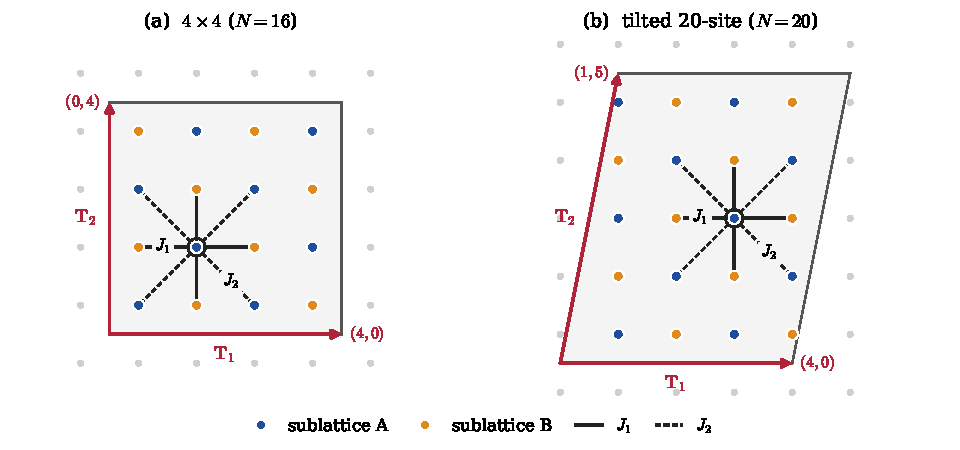
\includegraphics[width=0.8\textwidth]{fig1_lattices.pdf}
\caption{Exact clusters with periodic boundaries: (a) $4\times4$, (b) tilted
20-site torus. Colours: Marshall sublattices; arrows: periodic vectors;
$J_1$/$J_2$ bonds shown for one site.}
\label{fig:lattices}
\end{figure}
\end{widetext}

\section{Results}
\label{sec:results}
% TODO: text

\subsection{Krylov sign update}
% TODO: text

\subsubsection{Exact amplitude}
% TODO: text

\begin{widetext}
\begin{figure}[H]
\centering
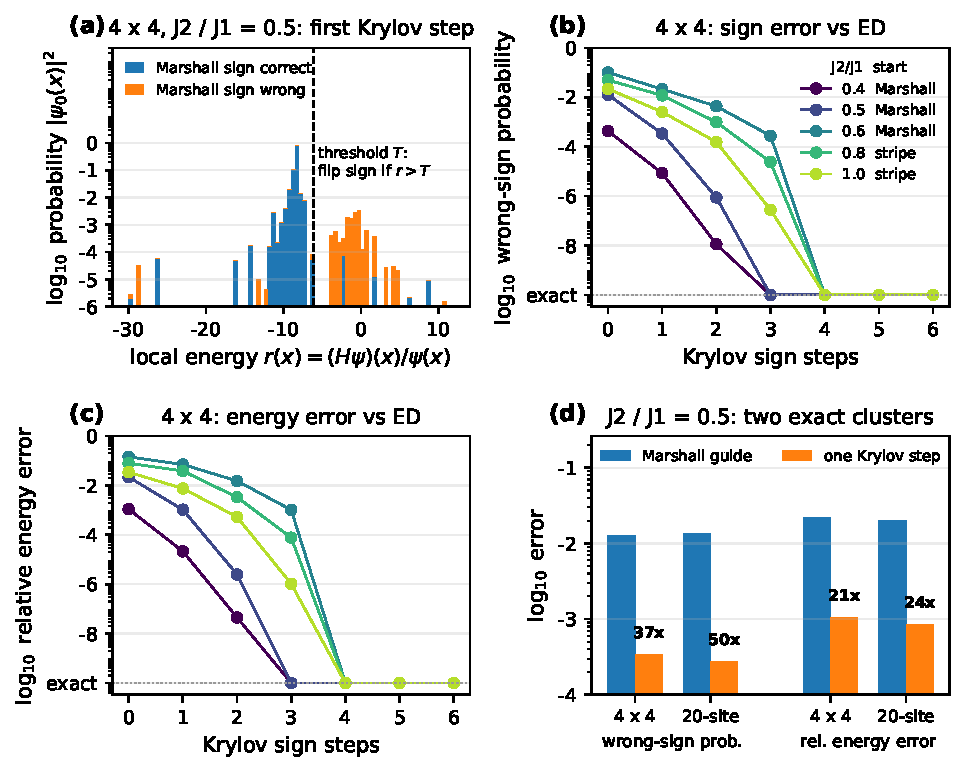
\includegraphics[width=\textwidth]{fig2_krylov_exact_amp.pdf}
\caption{Sign correction by Krylov steps, starting from Marshall signs. Only
the signs change; the amplitude stays the exact ED one. (a) $r(x)$ at
$J_2/J_1=0.5$; dashed line: threshold $T$. (b) Wrong-sign probability and
(c) energy error vs number of Krylov sign steps, compared with ED. (d) First
step on the $4\times4$ and 20-site clusters (Fig.~\ref{fig:lattices}).}
\label{fig:proof}
\end{figure}
\end{widetext}

\subsubsection{Approximate amplitude}
% TODO: text

\begin{widetext}
\begin{figure}[H]
\centering
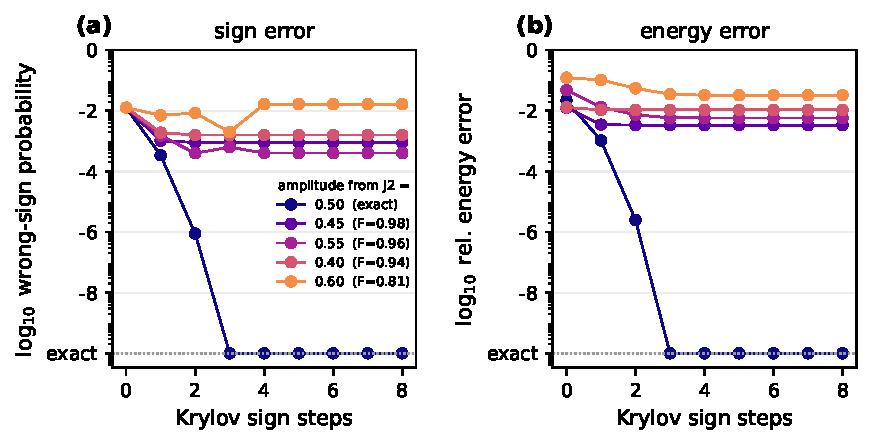
\includegraphics[width=0.85\textwidth]{fig3_krylov_approx_amp.pdf}
\caption{Krylov sign steps on an approximate amplitude at $J_2/J_1=0.5$; the
amplitude is the exact one of $J_2'$ (fidelity $F$). (a) Sign and (b) energy
error vs number of Krylov sign steps, compared with ED.}
\label{fig:approx}
\end{figure}
\end{widetext}

\subsubsection{Neural-network amplitude on $6\times6$}
\label{sec:vit6}
% TODO: text

\begin{widetext}
\begin{figure}[H]
\centering
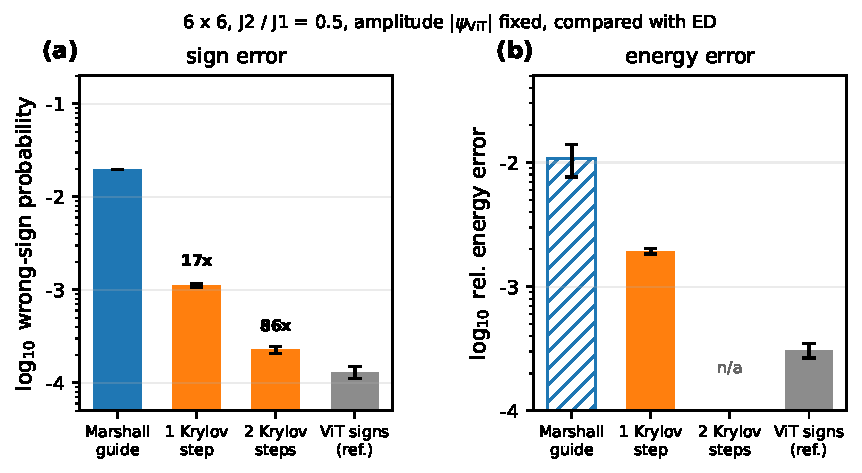
\includegraphics[width=0.9\textwidth]{fig4_krylov_vit_6x6.pdf}
\caption{Krylov sign steps on the ViT amplitude ($6\times6$), compared with ED,
with the ViT's own signs as reference. (a) Wrong-sign probability
($4\times10^5$ exact samples). (b) Relative energy error; the Marshall value
(hatched) is a lower bound from a smaller sample, the two-step energy is not
resolved.}
\label{fig:vit6}
\end{figure}
\end{widetext}

\subsection{Fixed-node--Krylov loop}
\label{sec:loop}
% TODO: text

\begin{widetext}
\begin{figure}[H]
\centering
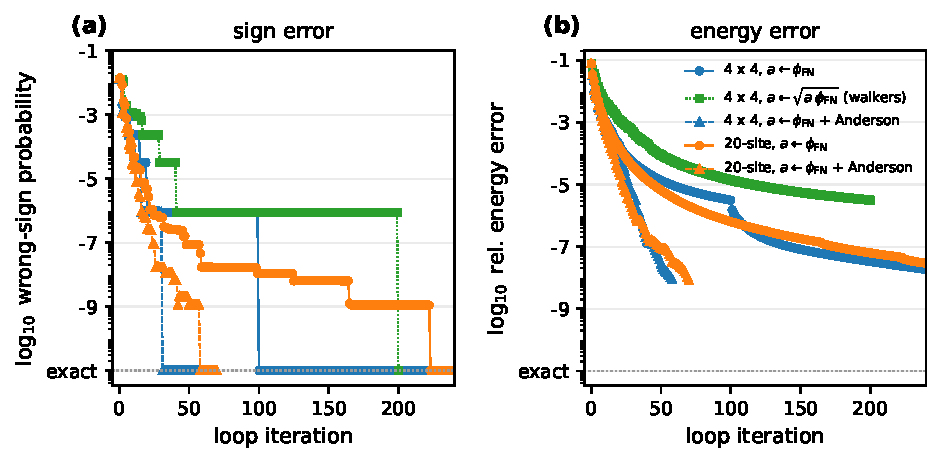
\includegraphics[width=0.85\textwidth]{fig5_fn_krylov_loop.pdf}
\caption{Fixed-node--Krylov loop with exact diagonalization, started from the
$J_2=0$ amplitude with Marshall signs, for three amplitude updates:
$a\leftarrow\phi_\FN$; $a\leftarrow\sqrt{a\,\phi_\FN}$, as learned from walkers;
and $a\leftarrow\phi_\FN$ with Anderson extrapolation from the last three iterates.
Dotted: Krylov steps alone from the same start, which change no sign.
(a) Sign and (b) energy error vs iteration, compared with ED. All values are
exact (no statistical error).}
\label{fig:closedloop}
\end{figure}
\end{widetext}

\subsection{Sampled fixed node on $4\times4$}
\label{sec:sampled4}
% TODO: text

\begin{widetext}
\begin{figure}[H]
\centering
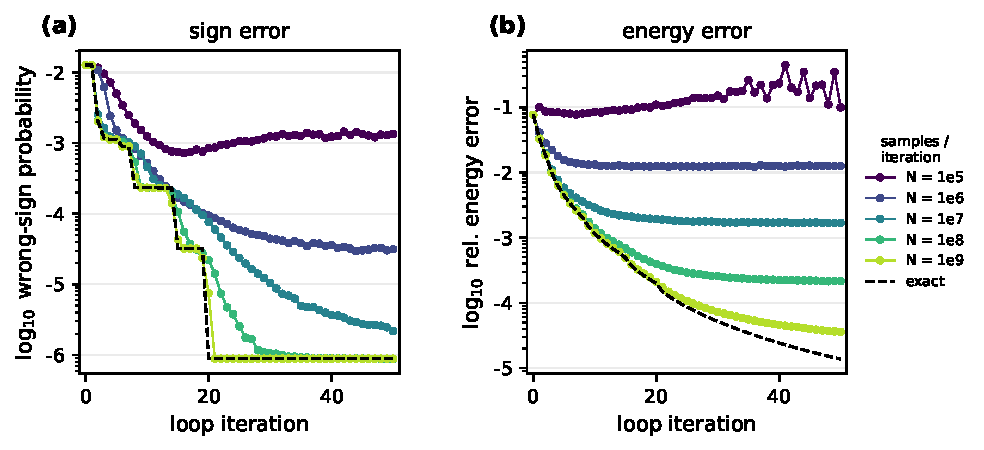
\includegraphics[width=0.9\textwidth]{fig6_sampled_4x4.pdf}
\caption{Fixed-node--Krylov loop on $4\times4$ with $\phi_\FN$ estimated from
$N$ independent samples per iteration (mean over four seeds; two for
$N=10^9$), and the exact loop. (a) Sign and (b) energy error vs iteration,
compared with ED.}
\label{fig:sampled}
\end{figure}
\end{widetext}

\subsection{First iteration at scale: $6\times6$ and $8\times8$}
% TODO: text

\begin{widetext}
\begin{figure}[H]
\centering
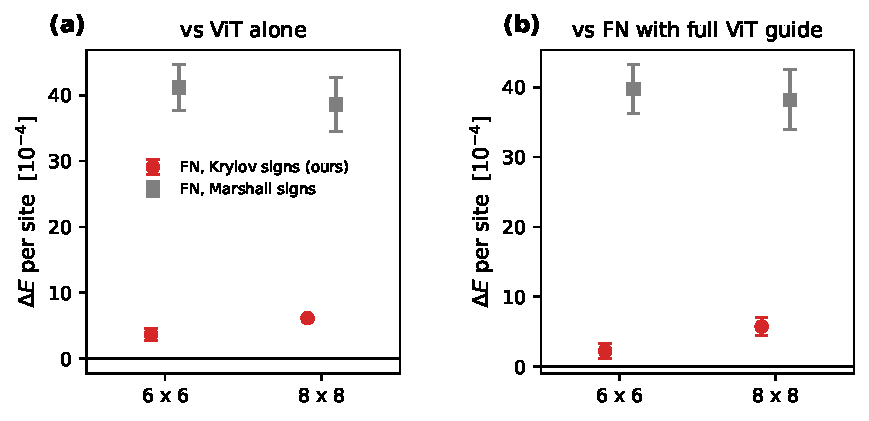
\includegraphics[width=0.85\textwidth]{fig7_guides_compare.pdf}
\caption{One untrained iteration on $6\times6$ and $8\times8$: fixed-node
energy with Krylov or Marshall signs on the ViT amplitude, relative to (a) the
ViT variational energy and (b) fixed node with the full ViT guide.}
\label{fig:guides}
\end{figure}
\end{widetext}

\begin{widetext}
\begin{figure}[H]
\centering
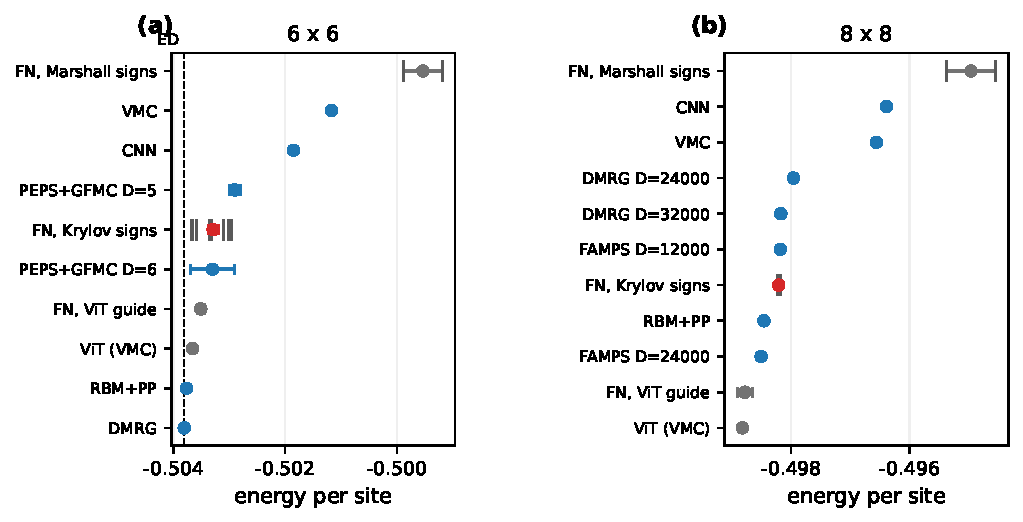
\includegraphics[width=\textwidth]{fig8_benchmarks.pdf}
\caption{Energies per site at $J_2/J_1=0.5$: our fixed-node values (Marshall,
Krylov, full ViT guide; $M=128$, not extrapolated), the ViT, and published
results: (a) $6\times6$, (b) $8\times8$. ED \cite{Schulz1996}, VMC
\cite{Hu2013}, CNN \cite{Choo2019}, DMRG \cite{Gong2014}, RBM+PP
\cite{NomuraImada2021}, PEPS+GFMC \cite{Lin2024}, FAMPS \cite{QianQin2023}.}
\label{fig:bench}
\end{figure}
\end{widetext}

\subsection{Closing the loop: learning the amplitude}
% TODO: text

\begin{widetext}
\begin{figure}[H]
\centering
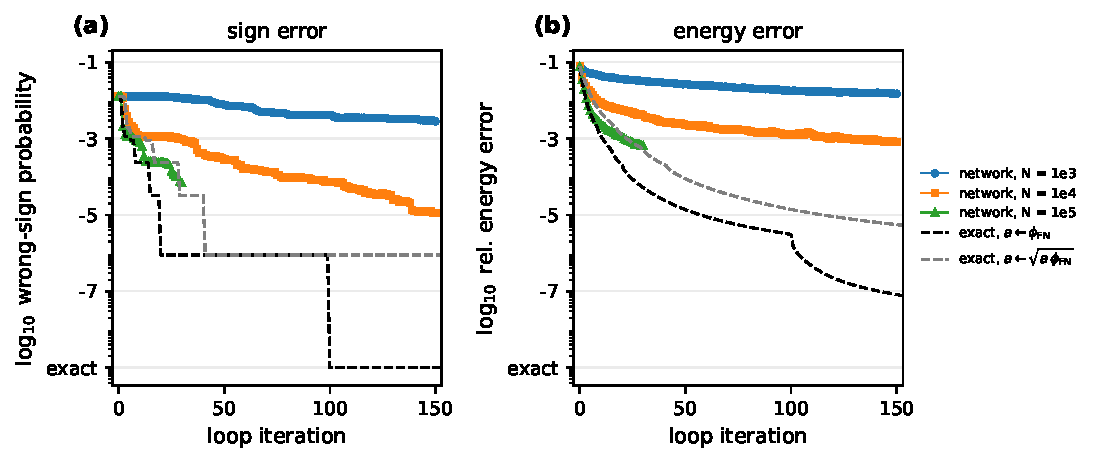
\includegraphics[width=\textwidth]{fig9_learning_4x4.pdf}
\caption{Fixed-node--Krylov loop on $4\times4$ with a network amplitude trained
on the frozen fixed-node energy from $N$ samples per SR step (mean over three
seeds), compared with the exact loops. (a) Sign and (b) energy error vs
iteration, compared with ED.}
\label{fig:learn4}
\end{figure}
\end{widetext}

\begin{widetext}
\begin{figure}[H]
\centering
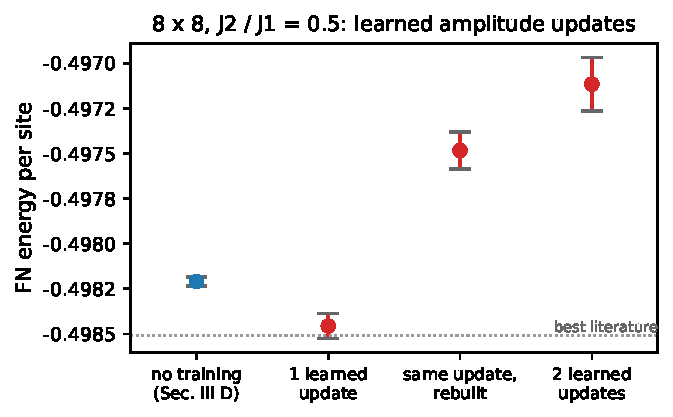
\includegraphics[width=0.6\textwidth]{fig10_learning_8x8.pdf}
\caption{$8\times8$ fixed-node energy per site along learned amplitude updates
(two walker populations each). Dotted: best same-geometry literature value
\cite{QianQin2023}.}
\label{fig:amplearn}
\end{figure}
\end{widetext}

\section{Discussion}
% TODO: text

\appendix

\section{Direct second Krylov step}
\label{app:k2}
% TODO: text

\section{Statistical conventions}
\label{app:stats}
% TODO: text

\bibliography{refs}
\end{document}